\documentclass{beamer}

\beamertemplatenavigationsymbolsempty

\mode<presentation>
{
  \usetheme{default}
}

\usepackage[english]{babel}
\usepackage[utf8]{inputenc}
\usepackage{bussproofs}
\usepackage[retainorgcmds]{IEEEtrantools}

 % for checkmark and cross
\usepackage{pifont}
\newcommand{\cmark}{\ding{51}}
\newcommand{\xmark}{\ding{55}}

% needs debian package texlive-math-extra
\usepackage{stmaryrd} % for \llbracket, \rrbracket

\usepackage{times}
\usepackage[T1]{fontenc}
% Or whatever. Note that the encoding and the font should match. If T1
% does not look nice, try deleting the line with the fontenc.

\usepackage{tikz}
\usetikzlibrary{positioning}
\usetikzlibrary{calc}
\usetikzlibrary{matrix}
\usetikzlibrary{arrows}


\newcommand{\product}{\!\times\!}
\newcommand{\aand}{\ \wedge \ }
\newcommand{\oor}{\ \vee \ }
\newcommand{\true}{\text{tt}}
\newcommand{\false}{\text{ff}}
\newcommand{\id}{\text{id}}
\newcommand{\fix}{\text{fix}}
\newcommand{\below}{\sqsubseteq}
\newcommand{\set}[1]{\{\,#1\,\}}
\newcommand{\bbN}{\mathbb{N}}
\newcommand{\lub}{\bigsqcup}
\newcommand{\Cppo}{\text{Cppo}}


\title
{Domains for Algebraic Data Types with Computation Steps}

\author
{Markus~Klinik}

\institute[Radboud University Nijmegen]
{
  Radboud University Nijmegen
}

\date
{August 2014}


\newcommand{\arr}{\rightarrow}
\newcommand{\Arr}{\Rightarrow}
\newcommand{\semantics}[1]{\llbracket #1 \rrbracket}
\newcommand{\semanticsFd}[1]{\semantics{#1}_{F\delta}}
\newcommand{\oftype}[2]{#1\!:\!#2}

\begin{document}

\begin{frame}
  \titlepage
\end{frame}



\begin{frame}{The Question}

\begin{center}
What is the connection between the functors

$1+X$

and

$1+X+X$?
\end{center}

\end{frame}



\begin{frame}{The Great Divide}

\begin{center}
"Love" is a four-letter word.
\end{center}

\end{frame}




\begin{frame}{PCF = $\lambda$++}


\begin{itemize}
\item untyped $\lambda$-calculus\onslide<2->{: fixpoint combinator}
\item simply typed $\lambda$-calculus\onslide<2->{: no fixpoints}
\item PCF\onslide<2->{: fixpoint operator}
\end{itemize}



%\setlength{\tabcolsep}{9pt}
%\renewcommand{\arraystretch}{1.3}
%\onslide<+->
%\begin{tabular}{c c c}
%untyped $\lambda$-calculus & typed $\lambda$-calculus & PCF \\
%\onslide<+->{fixpoint combinator & -- & fixpoint operator}
%\end{tabular}

\end{frame}


\begin{frame}{Fix}


\begin{center}

\onslide<+->
$Y\ M = M\ (Y\ M)$
\vspace{1em}

\onslide<+->
$\fix_t : (t \arr t) \arr t$
\vspace{1em}

$\fix\ M = M\ (\fix\ M)$
\vspace{1em}

\onslide<+->

$\fix\ M = M\ (\fix\ M) = M\ M\ (fix\ M) = M\ M\ M\ (fix\ M) = \ldots$
\end{center}


\end{frame}



\begin{frame}{PCF Semantics}
\begin{itemize}
\item We want abstractions to denote functions.
\item Every function must have a fixpoint.
\item Functions are partial.
\end{itemize}
\end{frame}

\begin{frame}{Scott's Fixpoint Semantics For Recursive Functions}

\begin{definition}
A \emph{partial order} is reflexive, transitive, antisymmetric.
\end{definition}

\begin{definition}
A \emph{complete pointed partial order} (cppo) is a
%\vspace{-1em}
\begin{itemize}
\item partial order where
\item every non-empty chain has a least upper bound
\item $\bot$ exists
\end{itemize}
\end{definition}

\begin{definition}
A \emph{continuous} function between cpos is monotone and preserves least upper bounds $f(\lub C) = \lub f(C)$
\end{definition}

\begin{theorem}[The Fixpoint Theorem]
Every continuous $f : D \arr D$ has a unique least fixpoint.
\end{theorem}

\end{frame}



\begin{frame}{The Fixpoint Theorem}

\begin{itemize} \itemsep0.5em
\onslide<+->
\item Let $D$ be a cppo, $f : D \arr D$ continuous.

\item $\bot \below f(\bot)
   \onslide<+->{ \below f(f(\bot))}
   \onslide<+->{\below f(f(f(\bot))) \below \ldots}$

\onslide<+->
\item $C = \set{f^n(\bot) \mid n \in \bbN}$ is a chain, has a least upper bound.

\onslide<+->
\item $f(C) = \set{f^{n+1}(\bot) \mid n \in \bbN}$

\onslide<+->
\item $\lub C = \lub f(C) = f(\lub C)$

\end{itemize}

\end{frame}



\begin{frame}[fragile]{PCF Semantics}

This lends itself well to the semantics:
\begin{itemize}
\item Types: complete pointed partial orders (cppos)
\item Abstraction: continuous functions between them
\end{itemize}

\vspace{1em}

\begin{tabular}{c c c}

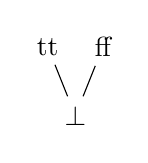
\begin{tikzpicture}
  \path (0,0) node [inner xsep=1em] {$\bot$} [grow'=up, sibling distance=2.0em, level distance=2.5em]
    child { node {tt} }
    child { node {ff} }
  ;
\end{tikzpicture}

&

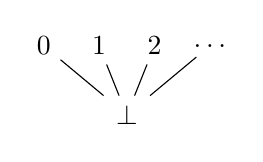
\begin{tikzpicture}
  \path (0,0) node [inner xsep=1em] {$\bot$} [grow'=up, sibling distance=2.0em, level distance=2.5em]
    child { node {$0$} }
    child { node {$1$} }
    child { node {$2$} }
    child { node {$\ldots$} edge from parent }
  ;
\end{tikzpicture}

&

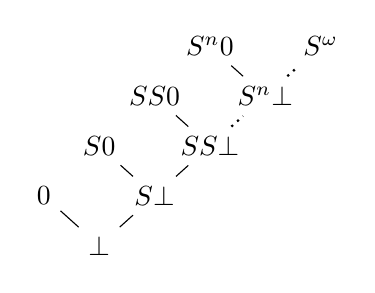
\begin{tikzpicture}[scale=1.0]
  \node {$\bot$} [grow'=up, sibling distance=4.0em, level distance=1.8em]
    child { node {$0$} }
    child
    {
      node {$S\bot$}
      child { node {$S0$} }
      child
      {
        node {$SS\bot$}
        child { node {$SS0$} }
        child [thick, dotted]
        {
          node {$S^n\bot$}
          child [thin, solid] { node {$S^n0$} }
          child { node {$S^\omega$} }
        }
      }
    }
  ;
\end{tikzpicture}

\end{tabular}

\end{frame}




\begin{frame}{Cppo}

\onslide<+->
In fact:
\begin{itemize}
\item Cppo: the category of cppos with continuous functions
\item Is a CCC: with products and exponentials
\item Has fixpoints: all endomorphisms have a fixpoint
\item But!
\end{itemize}


\end{frame}





\begin{frame}{Fixpoints, Sums, Products: Pick Two}

\begin{itemize}
\item What? CCC + Fixpoints + Coproducts = $\lightning$
\item Who? Huwig and Poign\'e, 1990
\item Why? Raising awareness
\item How? Let's see
\end{itemize}

\end{frame}




\begin{frame}[fragile]{Preliminaries}

\begin{definition}
A category is \emph{trivial} iff it has one object with one arrow.
\end{definition}

\begin{definition}
A category has \emph{fixpoints} iff every endomorphism has a fixpoint $Yf =
f(Yf)$
\end{definition}

\begin{center}
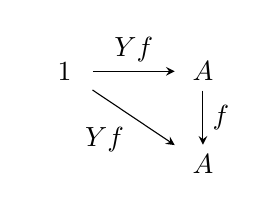
\begin{tikzpicture}
\matrix (m) [matrix of math nodes,row sep=2em,column sep=3em,minimum width=2em
            ,nodes={anchor=center}
            ]
  {
     1 & A \\
     {} & A \\
  };
  \path[-stealth] (m-1-1) edge node [above] {$Yf$} (m-1-2);
  \path[-stealth] (m-1-1) edge node [below left] {$Yf$} (m-2-2);
  \path[-stealth] (m-1-2) edge node [right] {$f$} (m-2-2);
\end{tikzpicture}
\end{center}

\end{frame}



\begin{frame}[fragile]{Warming Up (1)}

\begin{lemma}
In a category with fixpoints, $0 \cong 1$.
\end{lemma}

\vfill

\begin{center}
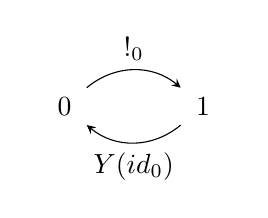
\begin{tikzpicture}
\matrix (m) [matrix of math nodes,row sep=2em,column sep=3em,minimum width=2em]
  {
     0 & 1 \\
  };
  \path[-stealth] (m-1-1) [out=40,in=140] edge node [above] {$!_0$} (m-1-2);
  \path[-stealth] (m-1-2) [out=220, in=320] edge node [below] {$Y(id_0)$} (m-1-1);
\end{tikzpicture}
\end{center}

\end{frame}



\begin{frame}[fragile]{Warming Up (2)}

\begin{lemma}
In a CCC with initial object, for all $A$, $0 \cong 0 \product A$.
\end{lemma}

Existence:
\begin{center}
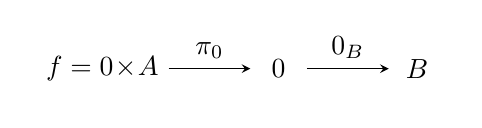
\begin{tikzpicture}
\matrix (m) [matrix of math nodes,row sep=4em,column sep=3em,minimum width=2em
            ,nodes={anchor=center}
            ]
  {
     f = 0 \product A & 0 & B \\
  };
  \path[-stealth] (m-1-1) edge node [above] {$\pi_0$} (m-1-2);
  \path[-stealth] (m-1-2) edge node [above] {$0_B$} (m-1-3);
\end{tikzpicture}
\end{center}

Uniqueness:
\begin{center}
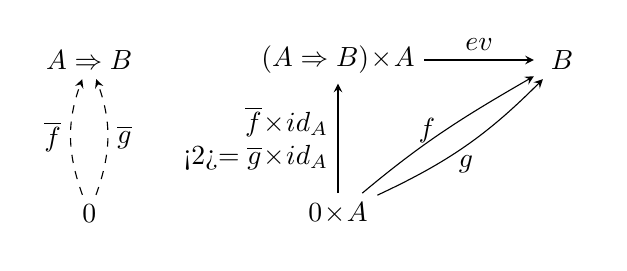
\begin{tikzpicture}
\matrix (m) [matrix of math nodes
            ,row sep=4em
            ,column sep=4em
            ,minimum width=2em
            ,nodes={anchor=center}
            ]
  {
     A \Arr B & (A \Arr B) \product A & B \\
     0 & 0 \product A \\
  };
  \path[-stealth, dashed] (m-2-1) [out=110,in=250] edge node [left] {$\overline{f}$} (m-1-1);
  \onslide<2->{\path[-stealth, dashed] (m-2-1) [out=70,in=290] edge node [right] {$\overline{g}$} (m-1-1);}
  \path[-stealth] (m-1-2) edge node [above] {$\text{ev}$} (m-1-3)
    (m-2-2) edge node [left,align=right] {$\overline{f} \product \id_A$\\{\onslide<2>{$= \overline{g} \product \id_A$}}} (m-1-2)
    (m-2-2) [out=40,in=210] edge node [left] {$f$} (m-1-3);
  \onslide<2->{\path[-stealth] (m-2-2) [out=25,in=225] edge node [below] {$g$} (m-1-3);}
\end{tikzpicture}
\end{center}

\end{frame}


\begin{frame}[fragile]{Warming Up (3)}

\begin{theorem}
Any CCC with fixpoints and initial object is trivial.
\end{theorem}

\begin{equation*}
1\ \cong\ 0\ \cong\ 0 \product A\ \cong\ 1 \product A\ \cong\ A
\end{equation*}

\end{frame}



\begin{frame}[fragile]{But Maybe Binary Sums?}

\begin{theorem}
Any CCC with fixpoints and binary sums is trivial.
\end{theorem}

\begin{lemma}
Any CCC with fixpoints and $1+1$ is trivial.
\end{lemma}

\end{frame}



\begin{frame}[fragile]{Boolean Algebra Objects}
Boolean algebra: $(B,\wedge,\vee,\neg,\true,\false)$ such that
\begin{itemize}
\item $\true = \neg \false$
\item $p = p \aand \true$
\item $\true = p \oor \neg p$
\item ...
\end{itemize}

Boolean algebra object: $(B,\ \wedge, \vee : B\product B \arr B,\ \neg : B \arr B,\ \true, \false : 1 \arr B)$ such that

\begin{center}
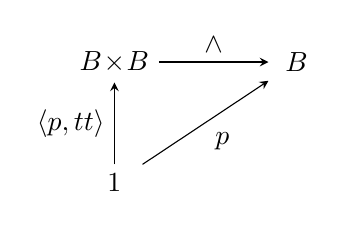
\begin{tikzpicture}
\matrix (m) [matrix of math nodes
            ,row sep=3em
            ,column sep=4em
            ,minimum width=2em
            ,nodes={anchor=center}
            ]
  {
     B \product B & B \\
     1 \\
  };
  \path[-stealth]
    (m-2-1) edge node [left] {$\langle p, \true \rangle$} (m-1-1)
    (m-1-1) edge node [above] {$\wedge$} (m-1-2)
    (m-2-1) edge node [below right] {$p$} (m-1-2) ;
\end{tikzpicture}
\end{center}

\end{frame}



\begin{frame}[fragile]{Why Boolean Algebra Objects?}

\begin{lemma}
The coproduct $1+1$ is a Boolean algebra object.
\end{lemma}

\begin{itemize}
\item $\true, \false$ are the coproduct inclusions $\kappa_0, \kappa_1 : 1 \arr 1+1$
\item $\neg$ is $[\kappa_1, \kappa_0] : 1+1 \arr 1+1$
\item ...
\end{itemize}

\begin{center}
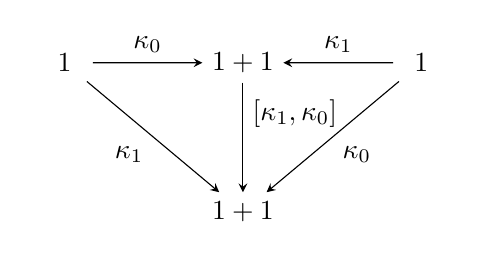
\begin{tikzpicture}[scale=1.2]
\matrix (m) [matrix of math nodes,row sep=4em,column sep=4em,minimum width=2em
            ,nodes={anchor=center}
            ]
  {
     1 & 1 + 1 & 1 \\
     {} & 1 + 1 & {} \\
  };
  \path[-stealth]
    (m-1-1) edge node [below left] {$\kappa_1$} (m-2-2)
            edge node [above] {$\kappa_0$} (m-1-2)
    (m-1-2) edge node [above right] {$[\kappa_1,\kappa_0]$} (m-2-2)
    (m-1-3) edge node [above] {$\kappa_1$} (m-1-2)
            edge node [below right] {$\kappa_0$} (m-2-2)
    ;
\end{tikzpicture}
\end{center}

\end{frame}


\begin{frame}[fragile]{Y Not}
If negation has a fixpoint we are in trouble:\\
Assume $Y \neg = \neg Y \neg$
\begin{IEEEeqnarray*}{rCl}
\true & = & Y\neg \oor \neg Y\neg \\
      & = & Y\neg \oor \phantom{\neg} Y\neg \\
      & = & Y\neg \\
      & = & Y\neg \aand \phantom{\neg} Y\neg \\
      & = & Y\neg \aand \neg Y\neg \\
      & = & \false
\end{IEEEeqnarray*}

In a category with fixpoints and $1+1$, $\neg$ has a fixpoint!\\
Thus $\kappa_0 = \kappa_1 : 1 \arr 1 + 1$
\end{frame}



\begin{frame}[fragile]{Adding Some More Equations}

\begin{itemize}
\item Fact: $- \product A$ preserves coproducts
\item $(1+1)\product A$ is a coproduct of $1 \product A$ and $1 \product A$
\item $(1+1) \product A\ \cong\ 2 \product A\ \cong\ A+A$
\item $A+A$ is a coproduct of $A$ and $A$ with $\kappa_0 \product A$ and $\kappa_1 \product A$
\item $\kappa_0 = \kappa_1 \implies \kappa_0 \product A = \kappa_1 \product A$
\end{itemize}


\begin{center}
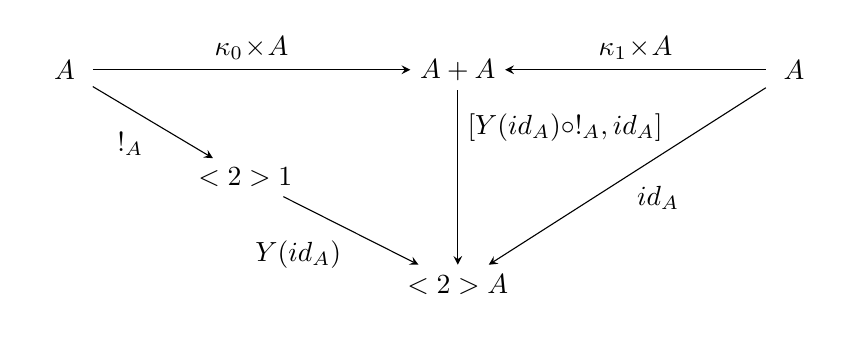
\begin{tikzpicture}
\matrix (m) [matrix of math nodes
            ,row sep=2.5em
            ,column sep=3.5em
            ,minimum width=2em
            ,nodes={anchor=center}
            ]
  {
     A & {} & A + A & {} & A \\
     {} & {\onslide<2>{1}} \\
     {} & {} & {\onslide<2>{A}} \\
  };
  \path[-stealth]
    (m-1-1) edge node [above] {$\kappa_0 \product A$} (m-1-3)
    (m-1-5) edge node [above] {$\kappa_1 \product A$} (m-1-3)
    ;
  \onslide<2>{\path[-stealth]
    (m-1-1) edge node [below left] {$!_A$} (m-2-2)
    (m-1-3) edge node [above=1.8em, right] {$[Y(\id_A) \circ !_A,\id_A]$} (m-3-3)
    (m-1-5) edge node [below right] {$\id_A$} (m-3-3)
    (m-2-2) edge node [below left] {$Y(\id_A)$} (m-3-3)
    ;}
\end{tikzpicture}
\end{center}


\end{frame}


\begin{frame}[fragile]{Conclusion, So Far}

\begin{center}
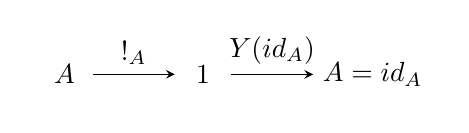
\begin{tikzpicture}
\matrix (m) [matrix of math nodes
            ,row sep=4em
            ,column sep=3em
            ,minimum width=2em
            ,nodes={anchor=center}
            ]
  {
     A & 1 & A = \id_A\\
  };
  \path[-stealth] (m-1-1) edge node [above] {$!_A$} (m-1-2);
  \path[-stealth] (m-1-2) edge node [above] {$Y(\id_A)$} (m-1-3);
\end{tikzpicture}
\end{center}

\begin{center}
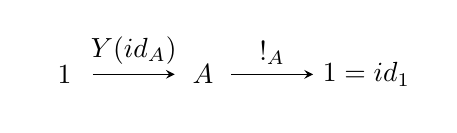
\begin{tikzpicture}
\matrix (m) [matrix of math nodes
            ,row sep=4em
            ,column sep=3em
            ,minimum width=2em
            ,nodes={anchor=center}]
  {
     1 & A & 1 = \id_1\\
  };
  \path[-stealth] (m-1-1) edge node [above] {$Y(\id_A)$} (m-1-2);
  \path[-stealth] (m-1-2) edge node [above] {$!_A$} (m-1-3);
\end{tikzpicture}
\end{center}

In every CCC with fixpoints and $1+1$, for all $A$, $A \cong 1$.

\end{frame}



\begin{frame}{Algebraic Data Types}

The essence of data:
\begin{itemize}
\item Products
\item Sums
\item Recursion
\end{itemize}
\vspace{2em}

\texttt{List = Nil | Cons Int List}

\end{frame}



\begin{frame}{Polynomial Functors}

A functor is polynomial iff it is of one of the forms
\begin{itemize}
\item Constant: $FX = D; Ff = \id_D$
\item Identity: $FX = X; Ff = f$
\item Sum: $FX = HX + GX$
\item Product: $FX = HX \product GX$
\end{itemize}

\end{frame}



\begin{frame}[fragile]{Denotational Semantics for Function Types}

Denotational Semantics depends on Operational Semantics:\\
Which function does this program denote?

\begin{center}

\onslide<+->
$\lambda x . 42$
\vspace{2em}

\onslide<+->
$x \mapsto 42$

\begin{equation*}
x \mapsto \left\{
  \begin{array}{lcl}
   42    & \text{if} & x \neq \bot \\
   \bot  & \text{if} & x = \bot
  \end{array}
\right.
\end{equation*}

\vspace{2em}
strict vs. non-strict functions

\end{center}

\end{frame}



\begin{frame}{Denotational Semantics for Product Types}

\onslide<+->
\begin{center}
$\pi_0 \langle M,N \rangle =\ ?$
\vspace{2em}

\onslide<+->
smash product: $\langle M, \bot\rangle = \bot = \langle\bot, N\rangle$

vs

cartesian product: $\langle M, \bot\rangle \neq \bot \neq \langle\bot, N\rangle$

\end{center}

\end{frame}


\begin{frame}{Denotational Semantics for Sum Types}

\onslide<+->
\begin{center}
$[\text{const}\ 42, \text{const}\ 43]\ \kappa_0(M) =\ ?$
\vspace{2em}

\onslide<+->
smash sum: $\kappa_0(\bot) = \bot = \kappa_1(\bot)$

vs

separated sum: $\kappa_0(\bot) \neq \bot \neq \kappa_1(\bot)$
\vspace{1.5em}

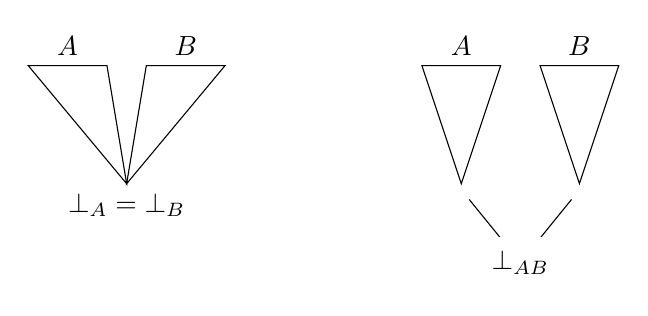
\begin{tikzpicture}[scale=1]
\draw (0,0) -- (0.5,0) node [above] {$A$} -- (1,0) -- (0.5,-1.5) -- cycle;
\begin{scope}[xshift=1.5cm]
\draw (0,0) -- (0.5,0) node [above] {$B$} -- (1,0) -- (0.5,-1.5) -- cycle;
\end{scope}
\draw[shape=rectangle] (0.6,-1.7) -- (1.25,-2.5)
  node [fill=white,inner sep=5pt] {$\bot_{AB}$} -- (1.9,-1.7)
;

\begin{scope}[xshift=-5cm]
\draw (0,0) -- (0.5,0) node [above] {$A$} -- (1,0) -- (1.25,-1.5) -- cycle;
\begin{scope}[xshift=1.5cm]
\draw (0,0) -- (0.5,0) node [above] {$B$} -- (1,0) -- (-0.25,-1.5)
  node [below] {$\bot_A = \bot_B$}
  -- cycle;
\end{scope}
\end{scope}

\end{tikzpicture}

\end{center}

\end{frame}



\begin{frame}{Summary So Far}

\begin{tabular}{c|c|c}
 & call-by-value & call-by-name \\
\hline
category & $\Cppo_{\bot}$ & $\Cppo$ \\
abstraction & strict cont. function & continuous function \\
sum type & smash sum & separated sum \\
product type & smash product & cartesian product \\
\end{tabular}

\end{frame}


\begin{frame}[fragile]{That's Okay Because}

\begin{itemize}
\item Separated sum not a coproduct in $\Cppo$
\item Smash product not a product in $\Cppo_\bot$
\end{itemize}
\vspace{1em}

\begin{center}
\begin{tabular}{l|c|c|c|c}
{} & CCC & fixpoints & bin. coproducts & initials \\
\hline
Problem & \cmark & \cmark & \cmark & \cmark \\
\hline
$\Cppo$ & \cmark & \cmark & \xmark & \xmark \\
\hline
$\Cppo_\bot$ & \xmark & \cmark & \cmark & \cmark \\
\end{tabular}
\end{center}

\end{frame}



\begin{frame}[fragile]{Clean}

Clean Language Report: ``Generic representations of ADTs are isomorphic to the original data types.''

\texttt{Three = A | B | C}
%\vspace{0.5em}

\onslide<2->{
\begin{center}
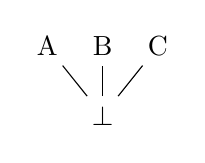
\begin{tikzpicture}
  \path (0,0) node [inner xsep=1em] {$\bot$} [grow'=up, sibling distance=2.0em, level distance=2.5em]
    child { node {A} }
    child { node {B} }
    child { node {C} }
  ;
\end{tikzpicture}
\end{center}
}
%\vspace{1em}

\texttt{ThreeG = Either (Either Unit Unit) Unit}
%\vspace{0.5em}

\onslide<2->{
\begin{center}
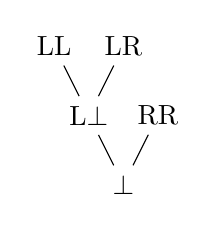
\begin{tikzpicture}
  \path (0,0) node [inner xsep=1em] {$\bot$} [grow'=up, sibling distance=2.5em, level distance=2.5em]
    child
    { node {L$\bot$}
      child { node {LL} }
      child { node {LR} }
    }
    child { node {RR} }
  ;
\end{tikzpicture}
\end{center}
}

\end{frame}


\begin{frame}{Why All This?}

\begin{itemize}
\item $\lambda^\arr$ is strongly normalizing
\item Gödel's System T is $\lambda^\arr$ plus
  \begin{itemize}
  \item natural numbers
  \item recursion operator
  \item primitive recursion
  \end{itemize}
\item Venanzio Capretta:
  \begin{itemize}
  \item coinductive natural numbers
  \item recursion operator
  \item general recursion
  \end{itemize}
\end{itemize}

\end{frame}



\begin{frame}{The Coinductive Natural Numbers}

Final coalgebra of the functor $1+X+X$

\begin{center}
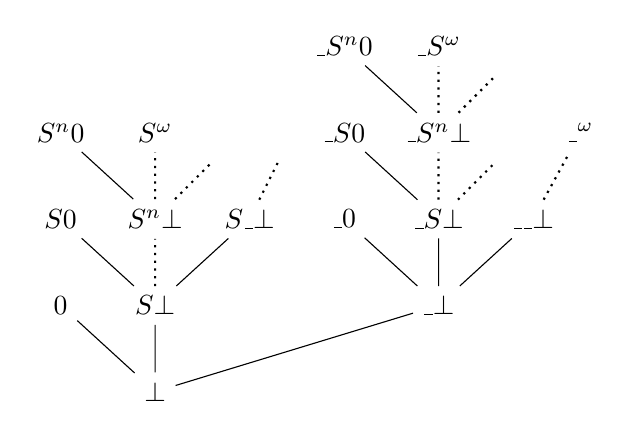
\begin{tikzpicture}
 [ grow'=up
 , scale=1.2
 , level distance=2.6em
 , level 1/.style={sibling distance=3cm}
 , level 2/.style={sibling distance=1cm}
 , normal/.style={thin, solid}
 , skipping/.style={thick, dotted}
 , and so on/.style={thick, dotted, sibling distance=0.6cm, level distance=0.6cm}
 ]
  \node {$\bot$}
    child [sibling distance=1cm] { node {$0$} }
    child
    {
      node {$S\bot$}
      child { node {$S0$} }
      child [skipping]
      {
        %node {$SS\bot$}
        %child { node {$SS0$} }
        %child [skipping]
        %{
          node {$S^n\bot$}
          child [normal] { node {$S^n0$} }
          child [skipping] { node {$S^\omega$} }
          child [and so on] {}
        %}
        %child [and so on] {}
      }
      child
      {
        node {$S\_\bot$}
        child [missing] {}
        child [and so on] {}
      }
    }
    child
    {
      node {$\_ \bot$}
      child { node {$\_0$} }
      child
      {
        node {$\_S\bot$}
        child { node {$\_S0$} }
        child [skipping]
        {
          node {$\_S^n\bot$}
          child [normal] { node {$\_S^n0$} }
          child { node {$\_S^\omega$} }
          child [and so on] {}
        }
        child [and so on] {}
      }
      child
      {
        node {$\_\_\bot$}
        child [missing] {}
        %child [missing] {}
        child [skipping] { node {$\_^\omega$} }
      }
    }
  ;
\end{tikzpicture}
\end{center}

\end{frame}




\begin{frame}{The Lazy Natural Numbers}

Final coalgebra of the functor $1+X$

\begin{center}
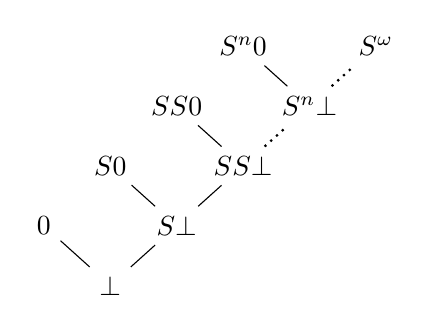
\begin{tikzpicture}[scale=1.2]
  \node {$\bot$} [grow'=up, sibling distance=4.0em, level distance=1.8em]
    child { node {$0$} }
    child
    {
      node {$S\bot$}
      child { node {$S0$} }
      child
      {
        node {$SS\bot$}
        child { node {$SS0$} }
        child [thick, dotted]
        {
          node {$S^n\bot$}
          child [thin, solid] { node {$S^n0$} }
          child { node {$S^\omega$} }
        }
      }
    }
  ;
\end{tikzpicture}
\end{center}

\end{frame}



\begin{frame}{What's Their Connection?}

\begin{center}
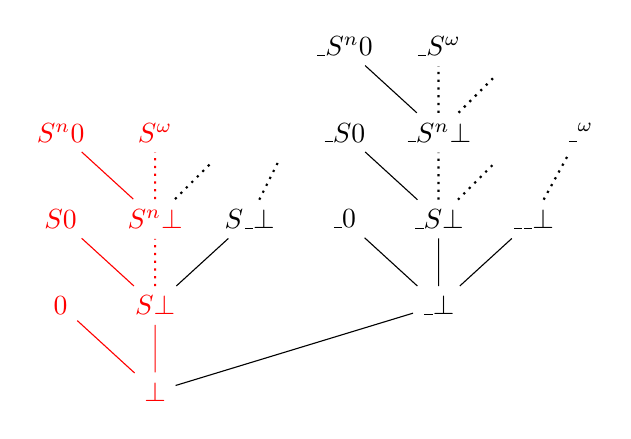
\begin{tikzpicture}
 [ grow'=up
 , scale=1.2
 , level distance=2.6em
 , level 1/.style={sibling distance=3cm}
 , level 2/.style={sibling distance=1cm}
 , normal/.style={thin, solid}
 , skipping/.style={thick, dotted}
 , and so on/.style={thick, dotted, sibling distance=0.6cm, level distance=0.6cm}
 ]
  \node [color=red] {$\bot$}
    child [sibling distance=1cm,color=red] { node [color=red] {$0$} }
    child [color=red]
    {
      node [color=red] {$S\bot$}
      child { node [color=red] {$S0$} }
      child [skipping]
      {
        %node {$SS\bot$}
        %child { node {$SS0$} }
        %child [skipping]
        %{
          node [color=red] {$S^n\bot$}
          child [normal,color=red] { node {$S^n0$} }
          child [skipping,color=red] { node {$S^\omega$} }
          child [and so on,color=black] {}
        %}
        %child [and so on] {}
      }
      child [color=black]
      {
        node {$S\_\bot$}
        child [missing] {}
        child [and so on] {}
      }
    }
    child
    {
      node {$\_ \bot$}
      child { node {$\_0$} }
      child
      {
        node {$\_S\bot$}
        child { node {$\_S0$} }
        child [skipping]
        {
          node {$\_S^n\bot$}
          child [normal] { node {$\_S^n0$} }
          child { node {$\_S^\omega$} }
          child [and so on] {}
        }
        child [and so on] {}
      }
      child
      {
        node {$\_\_\bot$}
        child [missing] {}
        %child [missing] {}
        child [skipping] { node {$\_^\omega$} }
      }
    }
  ;
\end{tikzpicture}
\end{center}

\end{frame}



\begin{frame}{Questions}
\begin{center}
?
\end{center}
\end{frame}


\end{document}
